\newpage
\section{Faraday Rotation}

\subsection{Execution}

\begin{figure}[!ht]
    \centering
    \includegraphics[width=0.85\textwidth]{img/setup3.png}
    \caption{Schematic of the setup used to record faraday rotation. As sample a WS$_2$ monolayer is used.}
    \label{fig_setup3}
\end{figure}
To measure the Faraday rotation of a WS$_2$ monolayer a novel setup by Dr. Ashish Arora and Dr. Benjamin Carey is used.
It is presented in \cref{fig_setup3} and allows a much faster acquisition of a whole spectrum than with previously used methods.
Here, two types of illumination ares used.
Firstly a laser to excite the monolayer and secondly a white light source to cover a broad energy spectrum rather than one energy at a time.
After polarizing the beam, it travels through the sample inside a magnetic field.
The transmitted light is then deflected into a lens system for reducing noise and focussing.
A key component in this setup is the beam displacer, where the beam splits into two.
This is dependent on the change in polarization induced by the sample.
Both beams are then each focused on a row on the CCD-chip, which acts as a spectrometer.
Again, to reduce noise the signals around the chosen rows are taken and subtracted as background.

\

According to the theoretical description in \cref{sec:theory}, measuring at a certain initial beam polarization allows us to obtain the Faraday rotation, however with background.
As this background does not change with the polarization, measurements are taken at \SI{+45}{\degree} and \SI{-45}{\degree} and then subtracted, since the Faraday rotation changes sign.

To ensure that the WS$_2$ monolayer is flat on a sapphire substrate, it is trapped between hexagonal boron nitride, which only adds a negligible contribution to the measured data.
Since the beam passes through both, the sapphire substrate and the WS$_2$ monolayer, again two measurements have to be taken do differentiate the background from the monolayer.
This is done by comparing the verdet constants of monolayer with substrate and of only substrate.

\subsection{Analysis}

\begin{figure}[!ht]
    \centering
    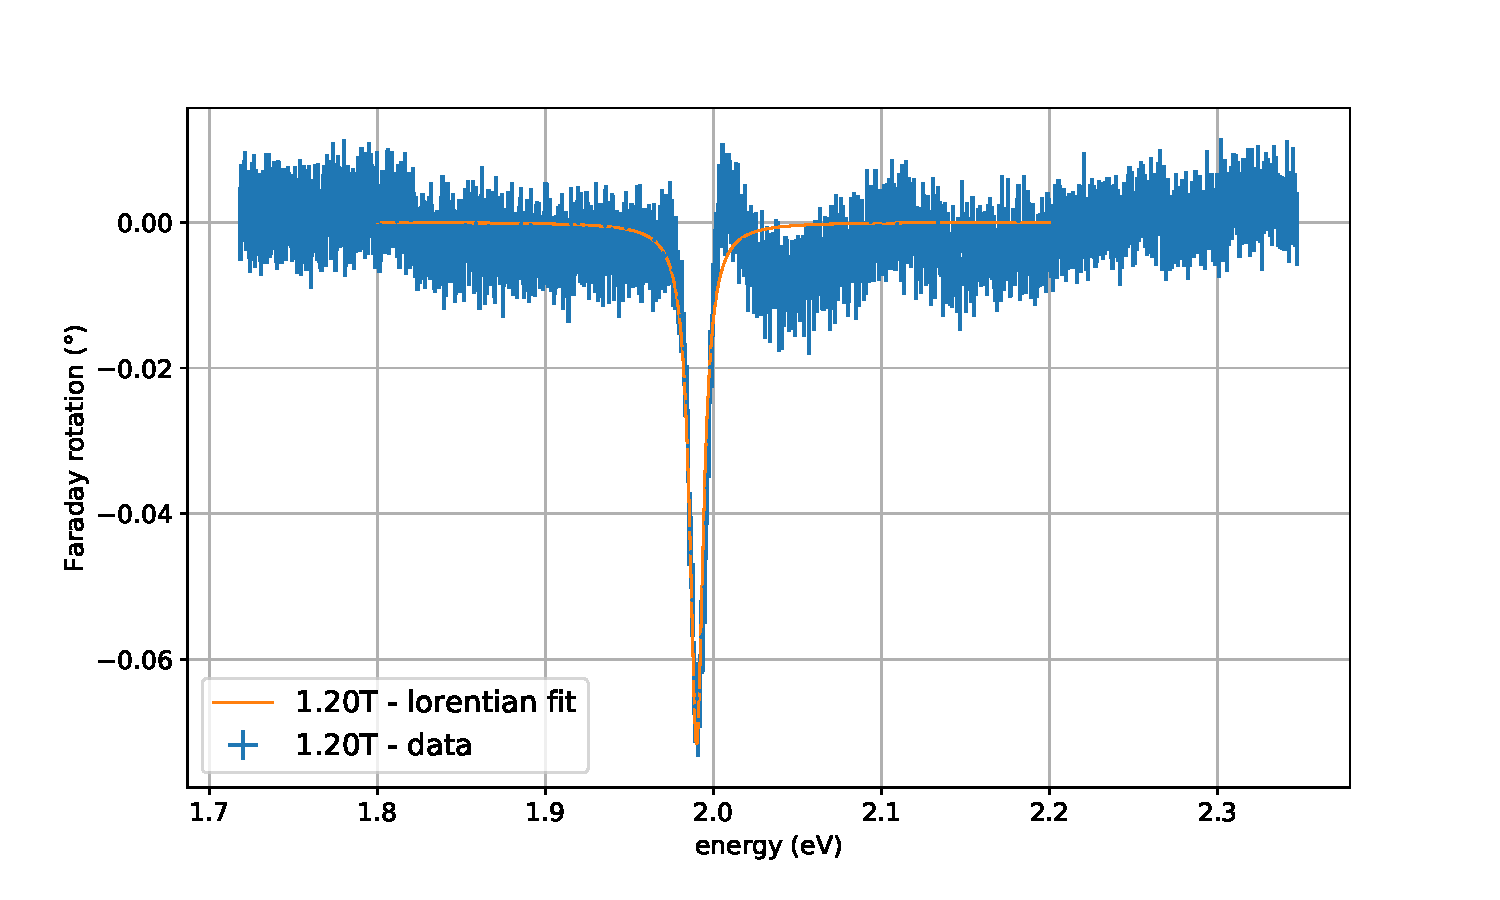
\includegraphics[width=0.85\textwidth]{plots/WS2_1200mT.pdf}
    \caption{Representation of WS$_2$ monolayer data points of the faraday rotation with external magnetic field of \SI{1.2}{\tesla} and lorentian fit.}
    \label{fig_WS2_1200mT}
\end{figure}
Since a lorentian line in the absorption spectrum is to be expected, lorentian fits are used for the data of the WS$_2$ monolayer.
An example is given in \cref{fig_WS2_1200mT} at \SI{1.2}{\tesla}.
All other plots of the data and their corresponding lorentian fits can be found in \cref{sec:appendix}.
Most of them fit very well with the data points, neglecting the noise.


\begin{figure}[!ht]
    \centering
    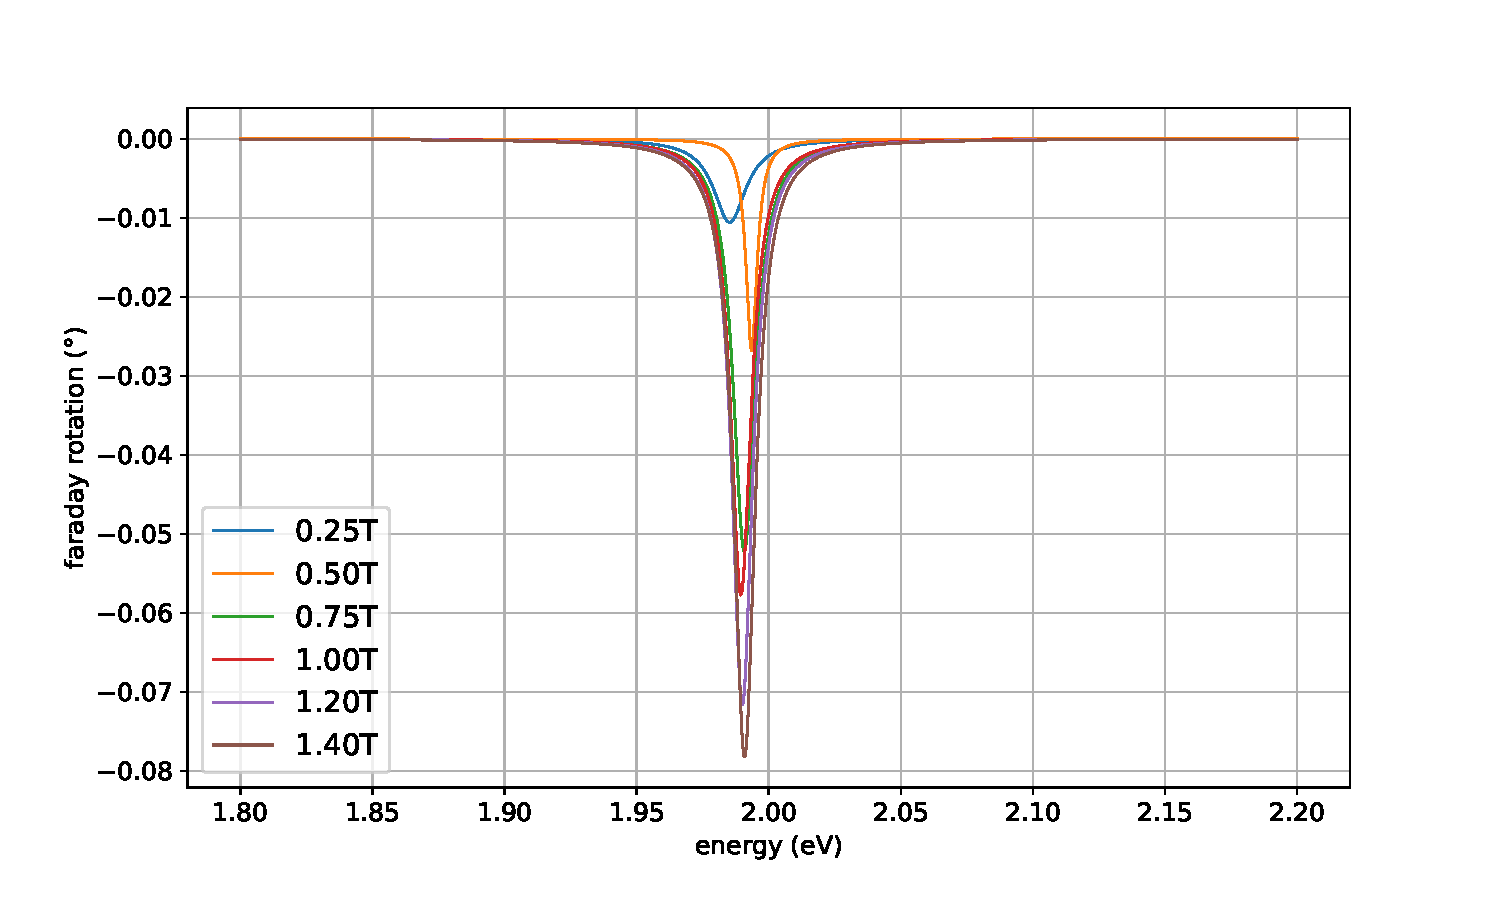
\includegraphics[width=0.85\textwidth]{plots/WS2_lorentians.pdf}
    \caption{Representation of all lorentian fits plotted together.}
    \label{fig_WS2_lorentians}
\end{figure}
For comparison all lorentian fits are found in \cref{fig_WS2_lorentians}.
As suspected an almost linear decrease if the value at the minimum can be seen.
Only the minimum at \SI{0.75}{\tesla} does not fit very well.
This may be due to remanent magnetisation, as the spectra were not taken in order of rising magnetic field strength.
Also, the energy of the minima is not exactly the same for all magnetic field strengths, as it should be.
However, since they are almost the same the mean value of \SI{}{} gives a good estimate. % TODO

\begin{figure}[!ht]
    \centering
    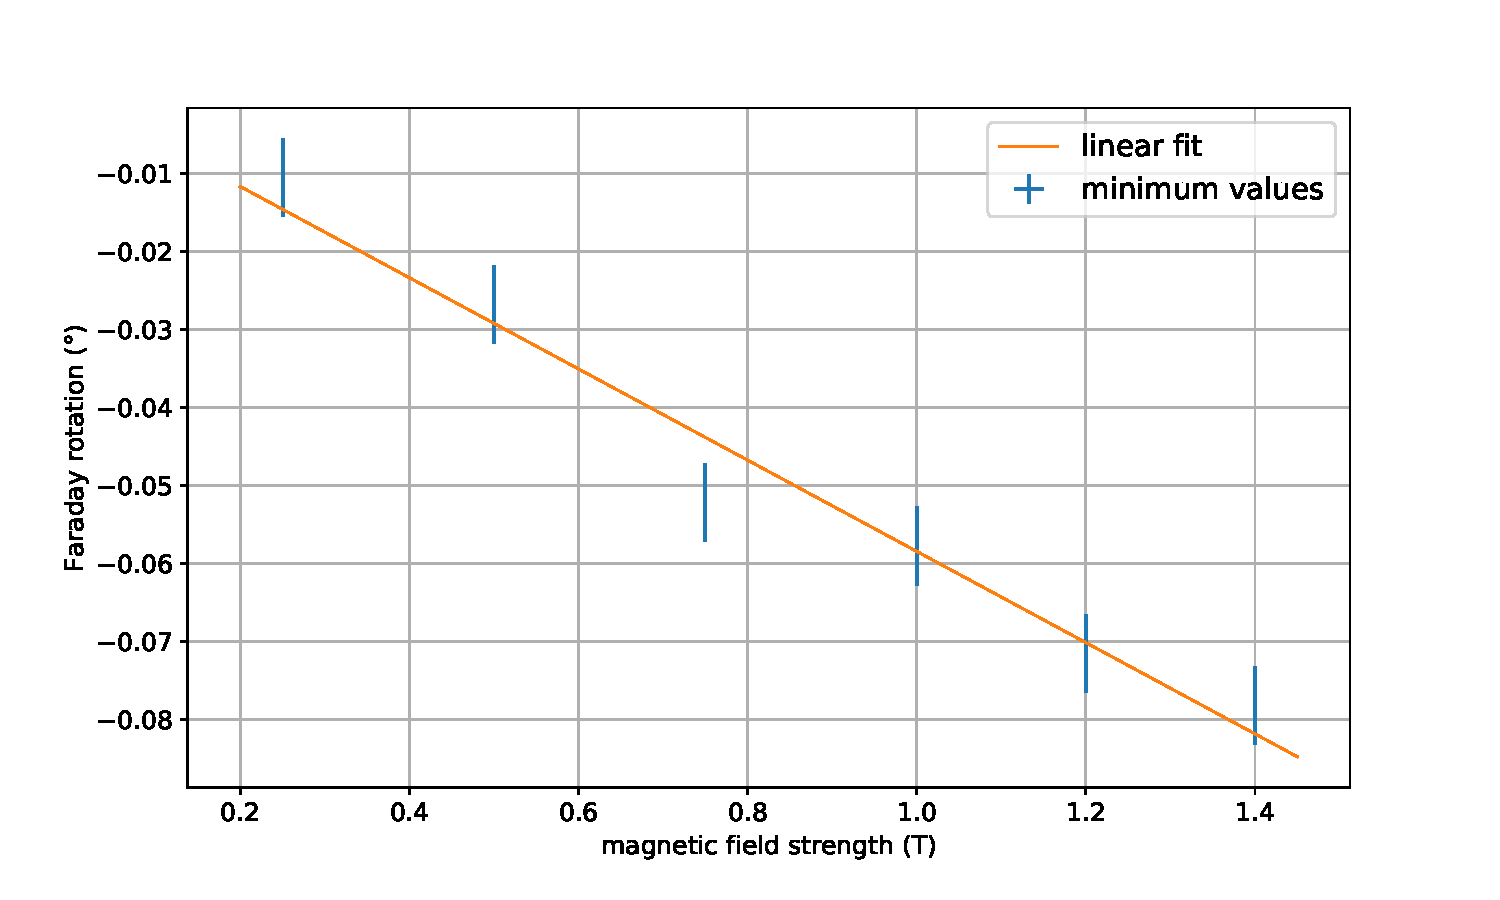
\includegraphics[width=0.85\textwidth]{plots/WS2_mins.pdf}
    \caption{Representation of largest WS$_2$s faraday rotation in dependence of external magnetic field strength.}
    \label{fig_WS2_minima}
\end{figure}
\cref{fig_WS2_minima} shows the beforementioned linear decrease by plotting the minima against the magnetic field strength.
Here, it also shows that the minimum at \SI{0.75}{\tesla} is a little of the expected value-

From its slope the verdet constant is extracted by division of the monolayers thickness of \SI{0.65}{\nano\meter}.
It amounts to \SI{}{}. % TODO

\

\begin{figure}[!ht]
    \centering
    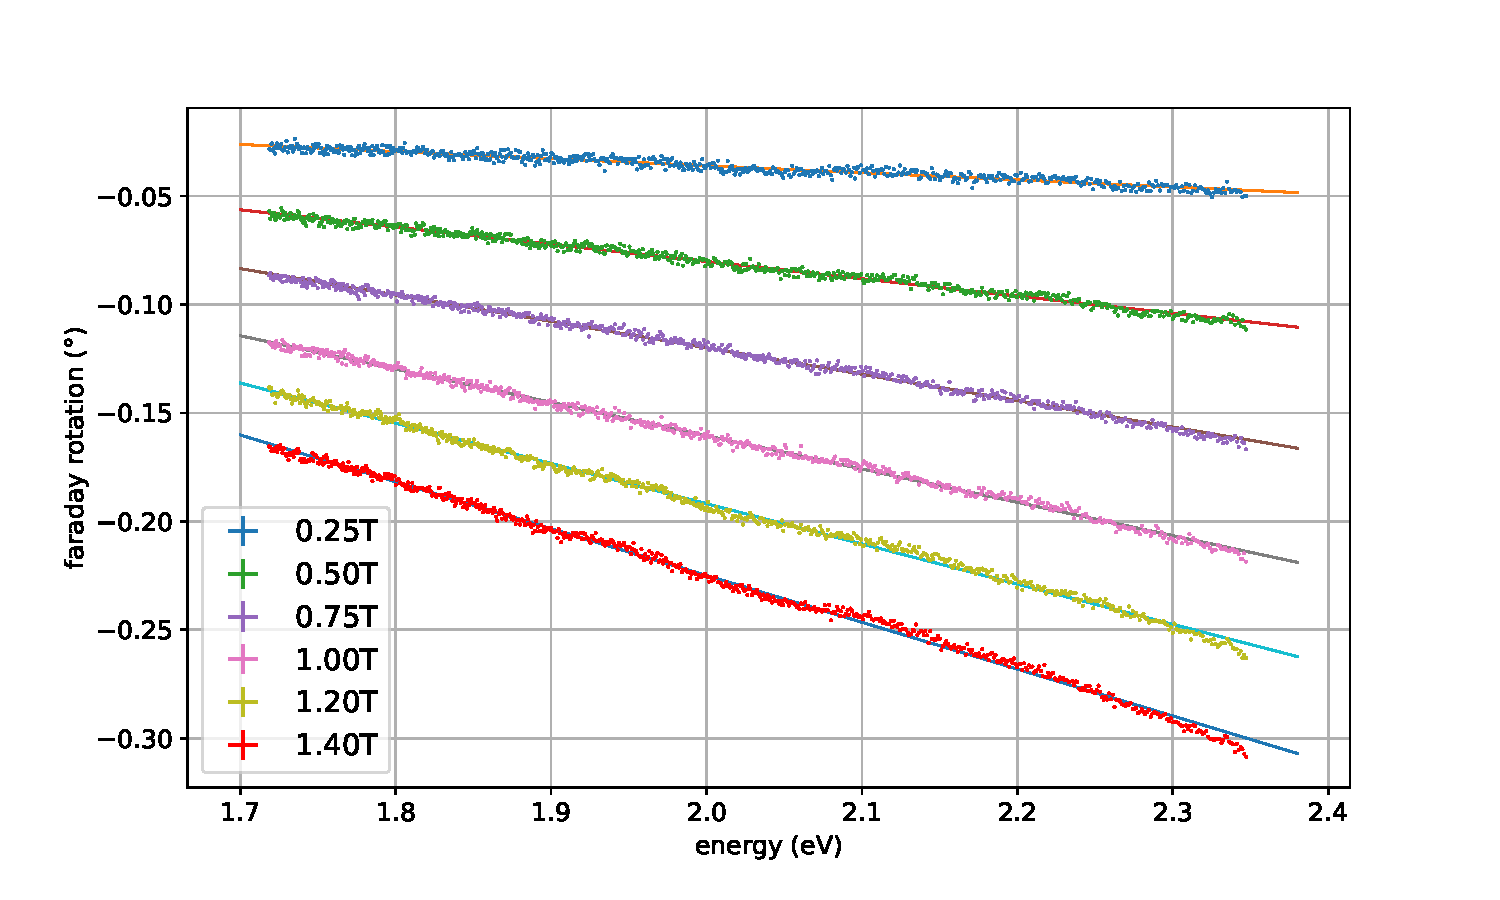
\includegraphics[width=0.85\textwidth]{plots/sapphire_lins.pdf}
    \caption{Representation of sapphire data points of the faraday rotation with different external magnetic fields and linear fits.}
    \label{fig_sapphire_lins}
\end{figure}
Contrary to the exciton contribution, only a linear decrease with rising energy is seen for the sapphire substrate in \cref{fig_sapphire_slopes}.
This linear decrease is fitted for each value of magnetic field strength.
The comparison of their slopes yet again shows another linear behavior.

\begin{figure}[!ht]
    \centering
    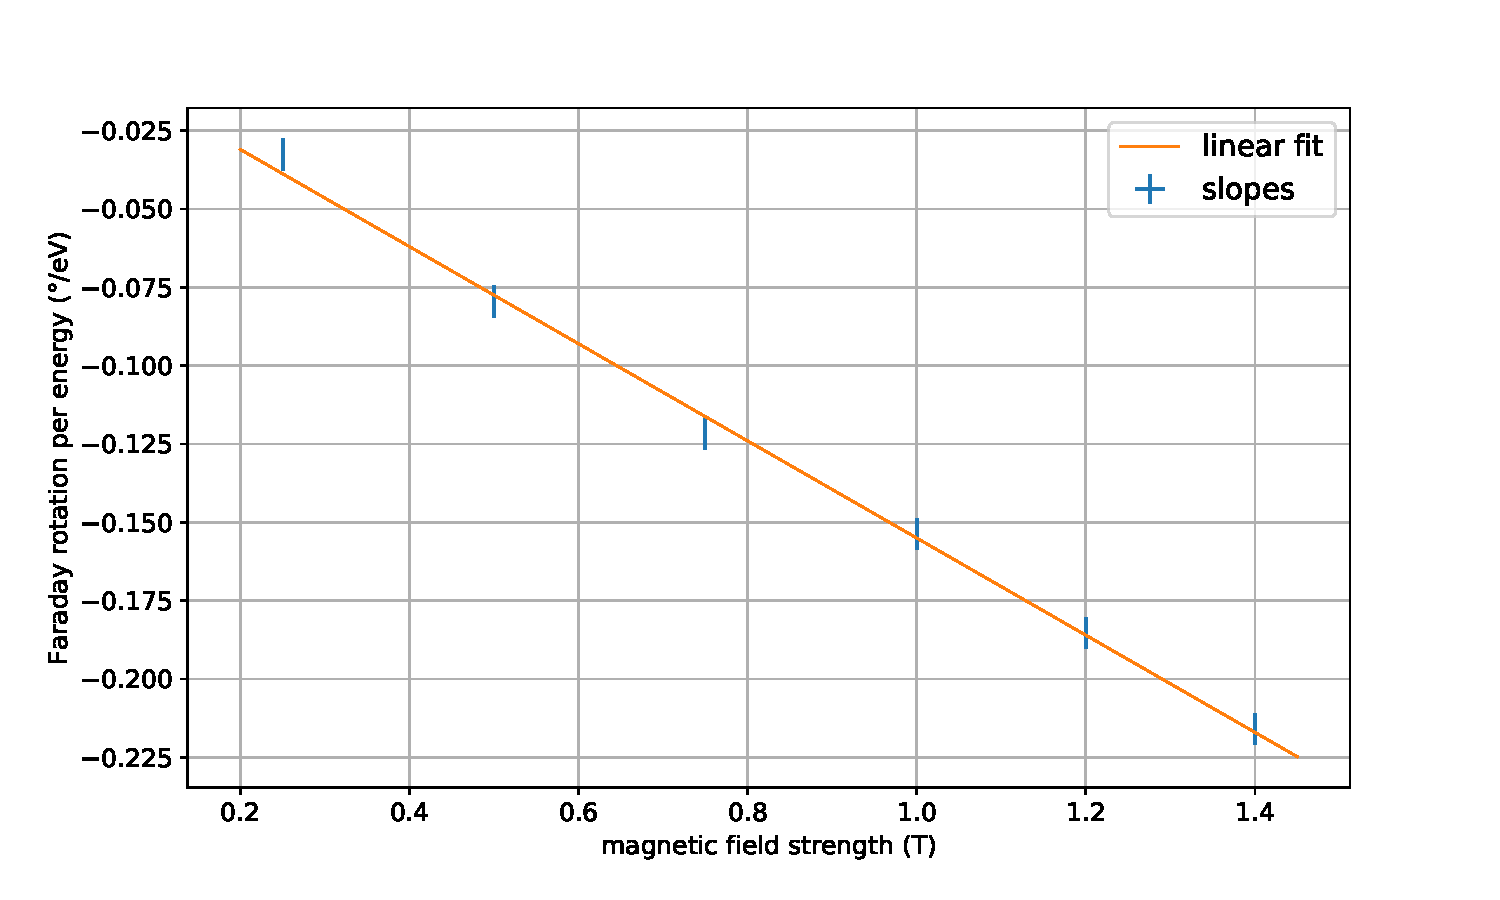
\includegraphics[width=0.85\textwidth]{plots/sapphire_slopes.pdf}
    \caption{Representation of sapphires faraday rotation in dependence of energy and external magnetic field strength.}
    \label{fig_sapphire_slopes}
\end{figure}
In \cref{fig_sapphire_lins} this is also fitted linearly.
Again by dividing this slope by the substrates thickness of \SI{0.5}{\milli\meter} the now energy dependent verdet constant of \SI{}{} is acquired.

To compare this value with the \SI{}{} of the WS$_2$ monolayer, it is multiplied with the energy of the minima and results in \SI{}{}.
These values differ in five orders of magnitude and thus show how strongly excitons influence the faraday rotation.
